% !TeX spellcheck = en_EN-English

\section{Prediction of record cost}
\label{costPredImple}

As discussed in Sec. \ref{recCostPred}, we used an MLP to predict the cost of a record. However, since our goal is to predict the future cost category of a patient and not the exact cost amount, we decided to also predict the cost category of the record instead of its precise cost.
\\

To assess how to split the interval of possible costs into sub-intervals corresponding to each category, we visualized the costs of records from our training dataset in a histogram. The resulting histogram can be seen in Fig. \ref{fig:cost_hist}, where the y-axis is linear and the x-axis is logarithmic, with the size of the bins also increasing logarithmically. From this, we can see that most records have costs between 0.1€ and 200€, so that is where we want most of the cost categories to be. We decided to merge all costs under one euro into a single category since, even though they are numerous, they have very little influence on the total cost of a patient in a year. Then, we split the interval between 1 and 200 into 6 categories with increasing width. After that, we grouped a few outliers between 200 and 500 into one category, and finally, we gave all outliers above 500 their own category. This gave us 9 categories, which are summarized in Tab. \ref{tab:cat_interval_record}.

\begin{figure}[!h]
	\centering
	
	% TODO image needs update with one computed from real training dataset
	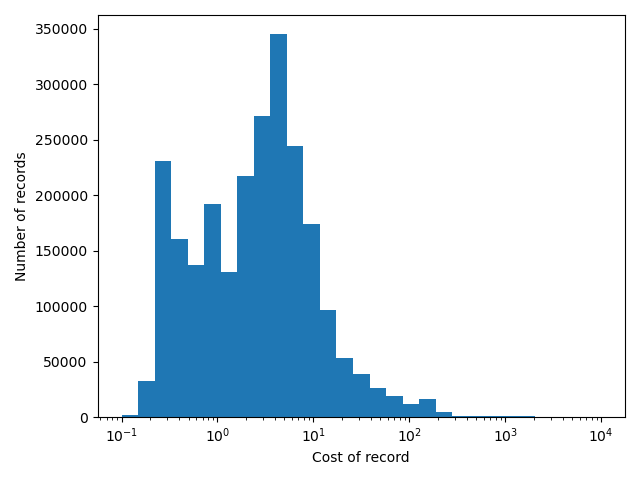
\includegraphics[width=0.8\textwidth]{images/cost_hist.png} 
	
	\caption{Histogram showing distribution of cost of records in training dataset.}
	\label{fig:cost_hist}
\end{figure} 

\begin{table}[!h]
	\centering
	\begin{tabular}{|l|l|}
		\hline
		Category  & Interval \\ \hline
		1 & $\interval[{0,1})$ \\ \hline
		2 & $\interval[{1,5})$ \\ \hline
		3 & $\interval[{5,10})$ \\ \hline
		4 & $\interval[{10,20})$ \\ \hline
		5 & $\interval[{20,50})$ \\ \hline
		6 & $\interval[{50,100})$ \\ \hline
		7 & $\interval[{100,200})$ \\ \hline
		8 & $\interval[{200,500})$ \\ \hline
		9 & $\interval[{500,\infty})$ \\ \hline
	\end{tabular}
	\caption{Intervals of record cost for each category.}
	\label{tab:cat_interval_record}
\end{table}  

The model itself consists of an input layer of size 196 (the final size of our embedding), followed by multiple linear layers with non-linear activation functions in between. This leads to a final layer of size 9 (matching the number of cost categories). The outputs of this final linear layer are passed through a softmax function to transform the raw values into probabilities for each category.
\\

We optimized multiple parameters of the network itself, as well as key training hyperparameters. From the perspective of the model architecture, we tested varying numbers of layers (model depth), their sizes, and the non-linear functions between them. For training, we experimented with three loss functions: mean squared error loss, cross-entropy loss, and negative log likelihood loss. As the optimizer, we chose Adaptive Moment Estimation (Adam) \cite{adam}, which adaptively adjusts learning rates during training and is considered an industry standard.
\\

Parameter selection was conducted by training multiple models on a smaller subset of the dataset locally. The final model was then trained with the chosen hyperparameters on the complete dataset using a server. All models were trained using a batch approach to limit the amount of data loaded at once, while avoiding gradient computation based solely on the loss from a single input (in this case, a single patient record).